\chapter{Технологическая часть}

\section{Выбор языка программирования и среды разработки.}

Для решения описанной задачи был выбран язык программирования - C\# \cite{Microsoft}.
Данный язык был выбран по следующим причинам:

\begin{itemize}
	\item он использует объектно-ориентированный подход к программированию,
	      что позволяет работать по принципу черного ящика;
	\item в языке присутствует обилие синтаксических возможностей,
	      которые помогают использовать готовые конструкции,
	      вместо того, чтобы переписывать однотипные строки кода;
	\item он имеет наличие большого количества библиотек и шаблонов,
	      позволяющих не тратить время на изобретение готовых конструкций;
	\item язык является строго типизированным,
	      что позволяет защититься от непроконтролированных ошибок;
	\item он является нативным, что необходимо
	      для увеличения скорости работы алгоритмов с помощью распараллеливания.
\end{itemize}

В качестве среды разработки был использован Visual Studio Code \cite{Vs}.
Visual Studio Code подходит не только для  Windows \cite{Win},
но и для Linux \cite{Lin}, это причина,
по которой был выбран VS code,
т.к. на моем компьютере установлена ОС Ubuntu 18.04.4 \cite{Ubuntu}.
Также моей архитектуре присутствует 8 ядер.

% \section{Сведения о модулях программы}
\section{Структура программы}

Данная программа состоит из следующих модулей:

\begin{itemize}
	\item Program.cs - файл, содержащий точку входа в программу.
	\item Vector.cs - файл, содержащий класс Vector, в котором
	      написаны основные методы для работы с вектором;
	\item Color.cs - файл, содержащий класс Color, в котором
	      написаны основные методы для работы с цветом;
	\item Constants.cs - файл, содержащий константы;
	\item Shape.cs - файл, содержащий базовый класс Shape
	      и унаследованные от него классы Sphere и Cylinder;
	\item Light.cs - файл, содержащий класс Light;
	\item MinForm.cs - файл, содержащий интерфейс и алгоритм трассировки лучей.
\end{itemize}

На рисунках \ref{fig:class_diagram1} - \ref{fig:class_diagram2} показана структура классов.

\begin{figure}[ht!]
	\centering{
		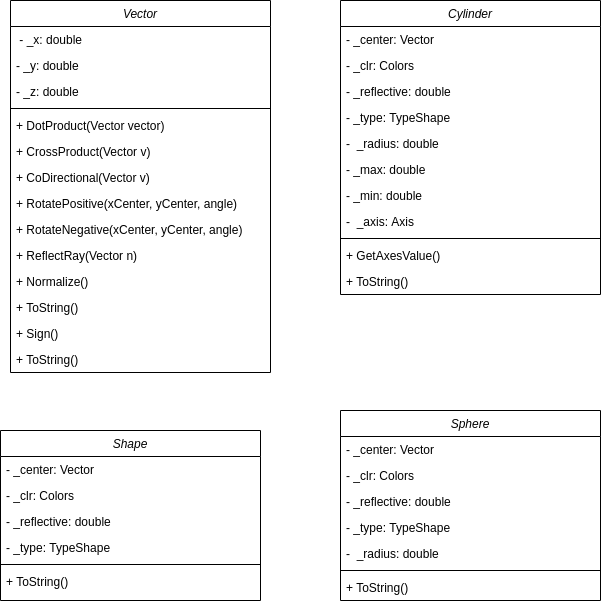
\includegraphics[width=0.5\textwidth]{class_diagram1.png}
		\caption{Структура классов}
		\label{fig:class_diagram1}}
\end{figure}

\begin{figure}[ht!]
	\centering{
		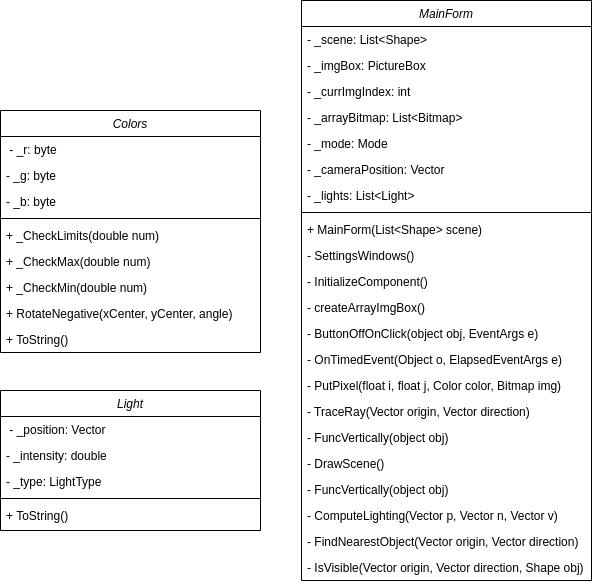
\includegraphics[width=0.5\textwidth]{class_diagram2.png}
		\caption{Структура классов}
		\label{fig:class_diagram2}}
\end{figure}

\newpage

На листинге 3.1 представлен основной код алгоритма.


\begin{lstlisting}[label=some-code,caption=Трассировка лучей.]
private Colors TraceRay(Vector origin, Vector direction, double min_t, double max_t, int depth = 3)
{
	double closest_t = Double.PositiveInfinity;
	Shape ClosestObject = FindNearestObject(origin, direction, min_t, max_t, ref closest_t);
	if (ClosestObject == null)
		return new Colors(0, 0, 0);

	Vector point = origin + direction * closest_t;
	Vector tmp = null;
	if (ClosestObject.Type == TypeShape.Sphere)
	{
		tmp = ClosestObject.Center;
	}
	else if (ClosestObject.Type == TypeShape.Cylinder)
	{
		Cylinder cylinder = ClosestObject as Cylinder;

		Vector axesValue = cylinder.GetAxesValue();   
		Vector axesValueRev = cylinder.GetAxesValue(); 		
		axesValueRev.Reverse();

		axesValue = axesValue * cylinder.Center; 
		axesValueRev = axesValueRev * point;
		tmp = axesValue + axesValueRev; 
	}

	Vector normal = point - tmp;
	normal = normal * (1.0d / normal.Length);
	Vector view = direction * -1.0d;
	double lighting = ComputeLighting(point, normal, view);

	Colors result = ClosestObject.Clr * lighting;

	if (depth <= 0)
		return result;

	Vector reflected_ray = ReflectRay(view, normal);
	Colors reflected_color = TraceRay(point, reflected_ray, 0.001d, Double.PositiveInfinity, depth - 1);

	double reflective = ClosestObject.Reflective;
	return result * (1 - reflective) + reflected_color * reflective;
}
\end{lstlisting}

\section{Вывод}

В данном разделе был выбран ЯП и среда разработки.
Также описаны модули и разобран листинг рис 3.1, показывающий работу алгоритма.